\documentclass[10pt]{article}
\usepackage[margin=0.75in]{geometry}
\usepackage{booktabs,graphicx,hyperref,xcolor}
\usepackage[T1]{fontenc}
\title{KO=0.5 Native-VC Brill Campaign and Experimental CPBC Assessment}
\author{AthenaK investigation handoff}
\date{26 August 2026}
\begin{document}
\maketitle
\section*{Verdict}
KO=0.5 does not yield a stable, convergent Figure-3 collapse evolution. The
matched-tree N128/N256/N512 campaign is near fourth order early, then loses
convergence first outside $r\le4M$ around the $\rho\simeq5M$ mode. N256 fails
at $t=14.405106M$ with an indefinite conformal metric after a catastrophic
noncentral runaway. N512 reaches the forced common stop but is also severely
unstable. The nonmonotone resolution ordering rules out convergence.

The common numerical curves end at central proper time 8.827, before the
published first peak near 10.31 and deep minimum near 12.62. Figure 3 is not
reproduced. The Cartoon constraint measure already uses
$2\pi\rho\sqrt{\gamma}\,d\rho\,dz$, so the jumps are not a collapsed-y
normalization artifact.

\section*{Matched-tree outcomes}
\begin{center}
\begin{tabular}{lrrr}
\toprule
Case & $C^2$ inventory & max $|\mathcal K|$ & $\Delta t$\\
\midrule
N128 & $2.344\times10^1$ & $9.441\times10^1$ & $2.888\times10^{-8}$\\
N256 & $2.677\times10^{18}$ & $8.434\times10^{30}$ & $5.615\times10^{-9}$\\
N512 & $1.774\times10^5$ & $4.244\times10^9$ & $3.081\times10^{-9}$\\
\bottomrule
\end{tabular}
\end{center}

All 141 noninitial hierarchy events replayed exactly. Early regional constraint
orders are close to four. At $t=8M$, $r\le4M$ remains near fourth order while
$r\le8M$ has already degraded, localizing the first loss of convergence outside
the center.

\begin{figure}[ht]
\centering
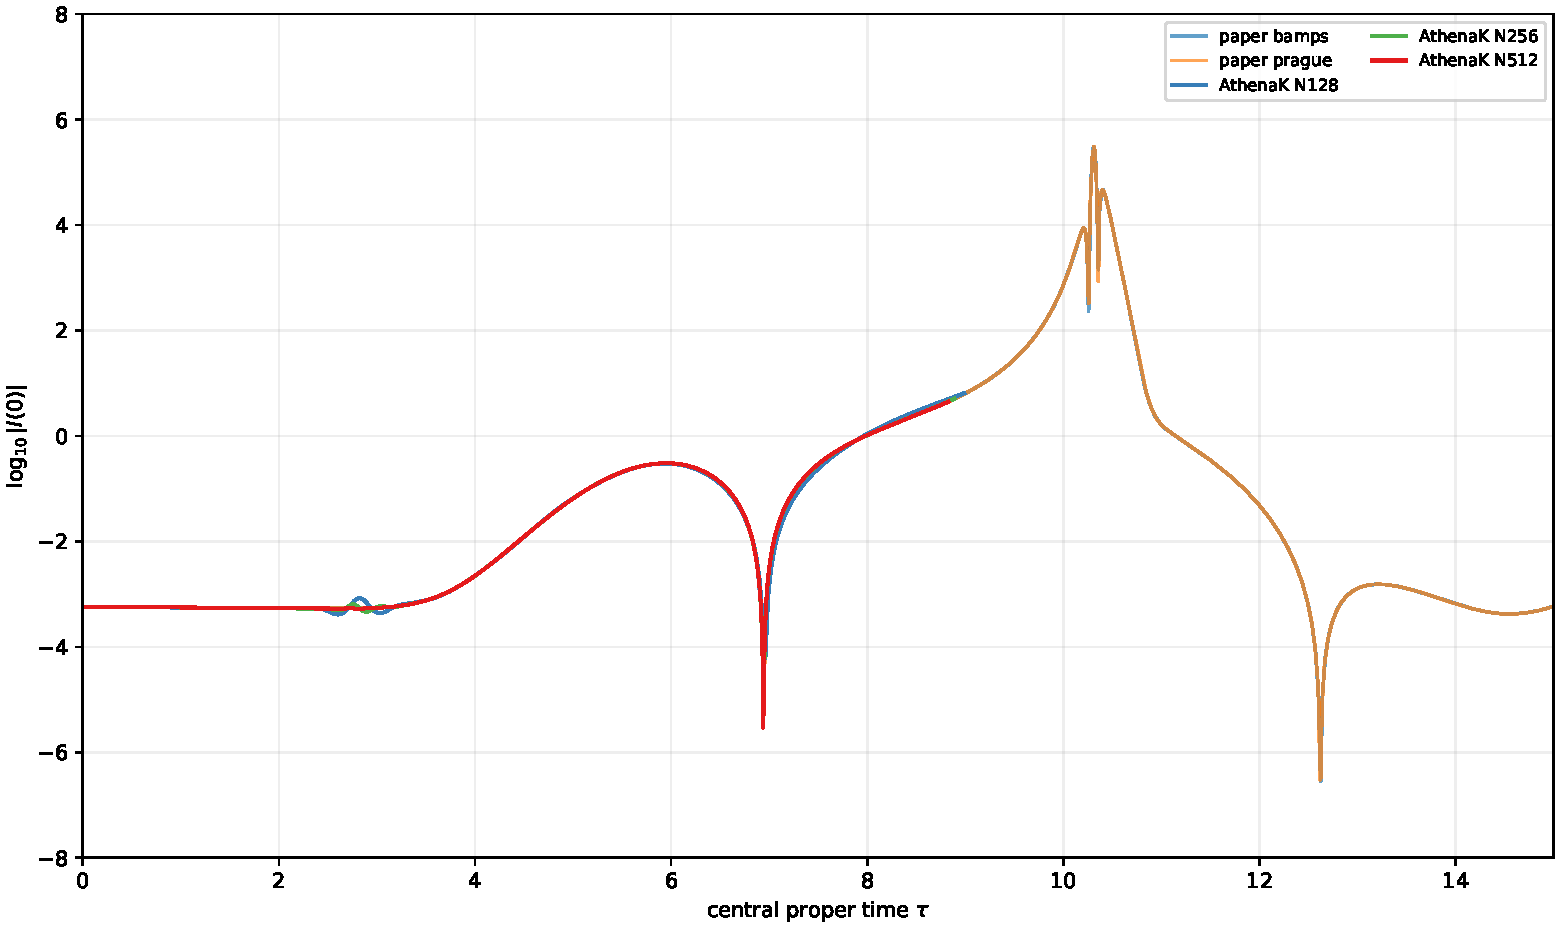
\includegraphics[width=.82\linewidth]{analysis/history/figures/figure3_three_resolution.pdf}
\caption{Published Figure-3 curves and the three AthenaK resolutions. No shifts
or rescalings are applied. The AthenaK interval ends before the first peak.}
\end{figure}

\begin{figure}[ht]
\centering
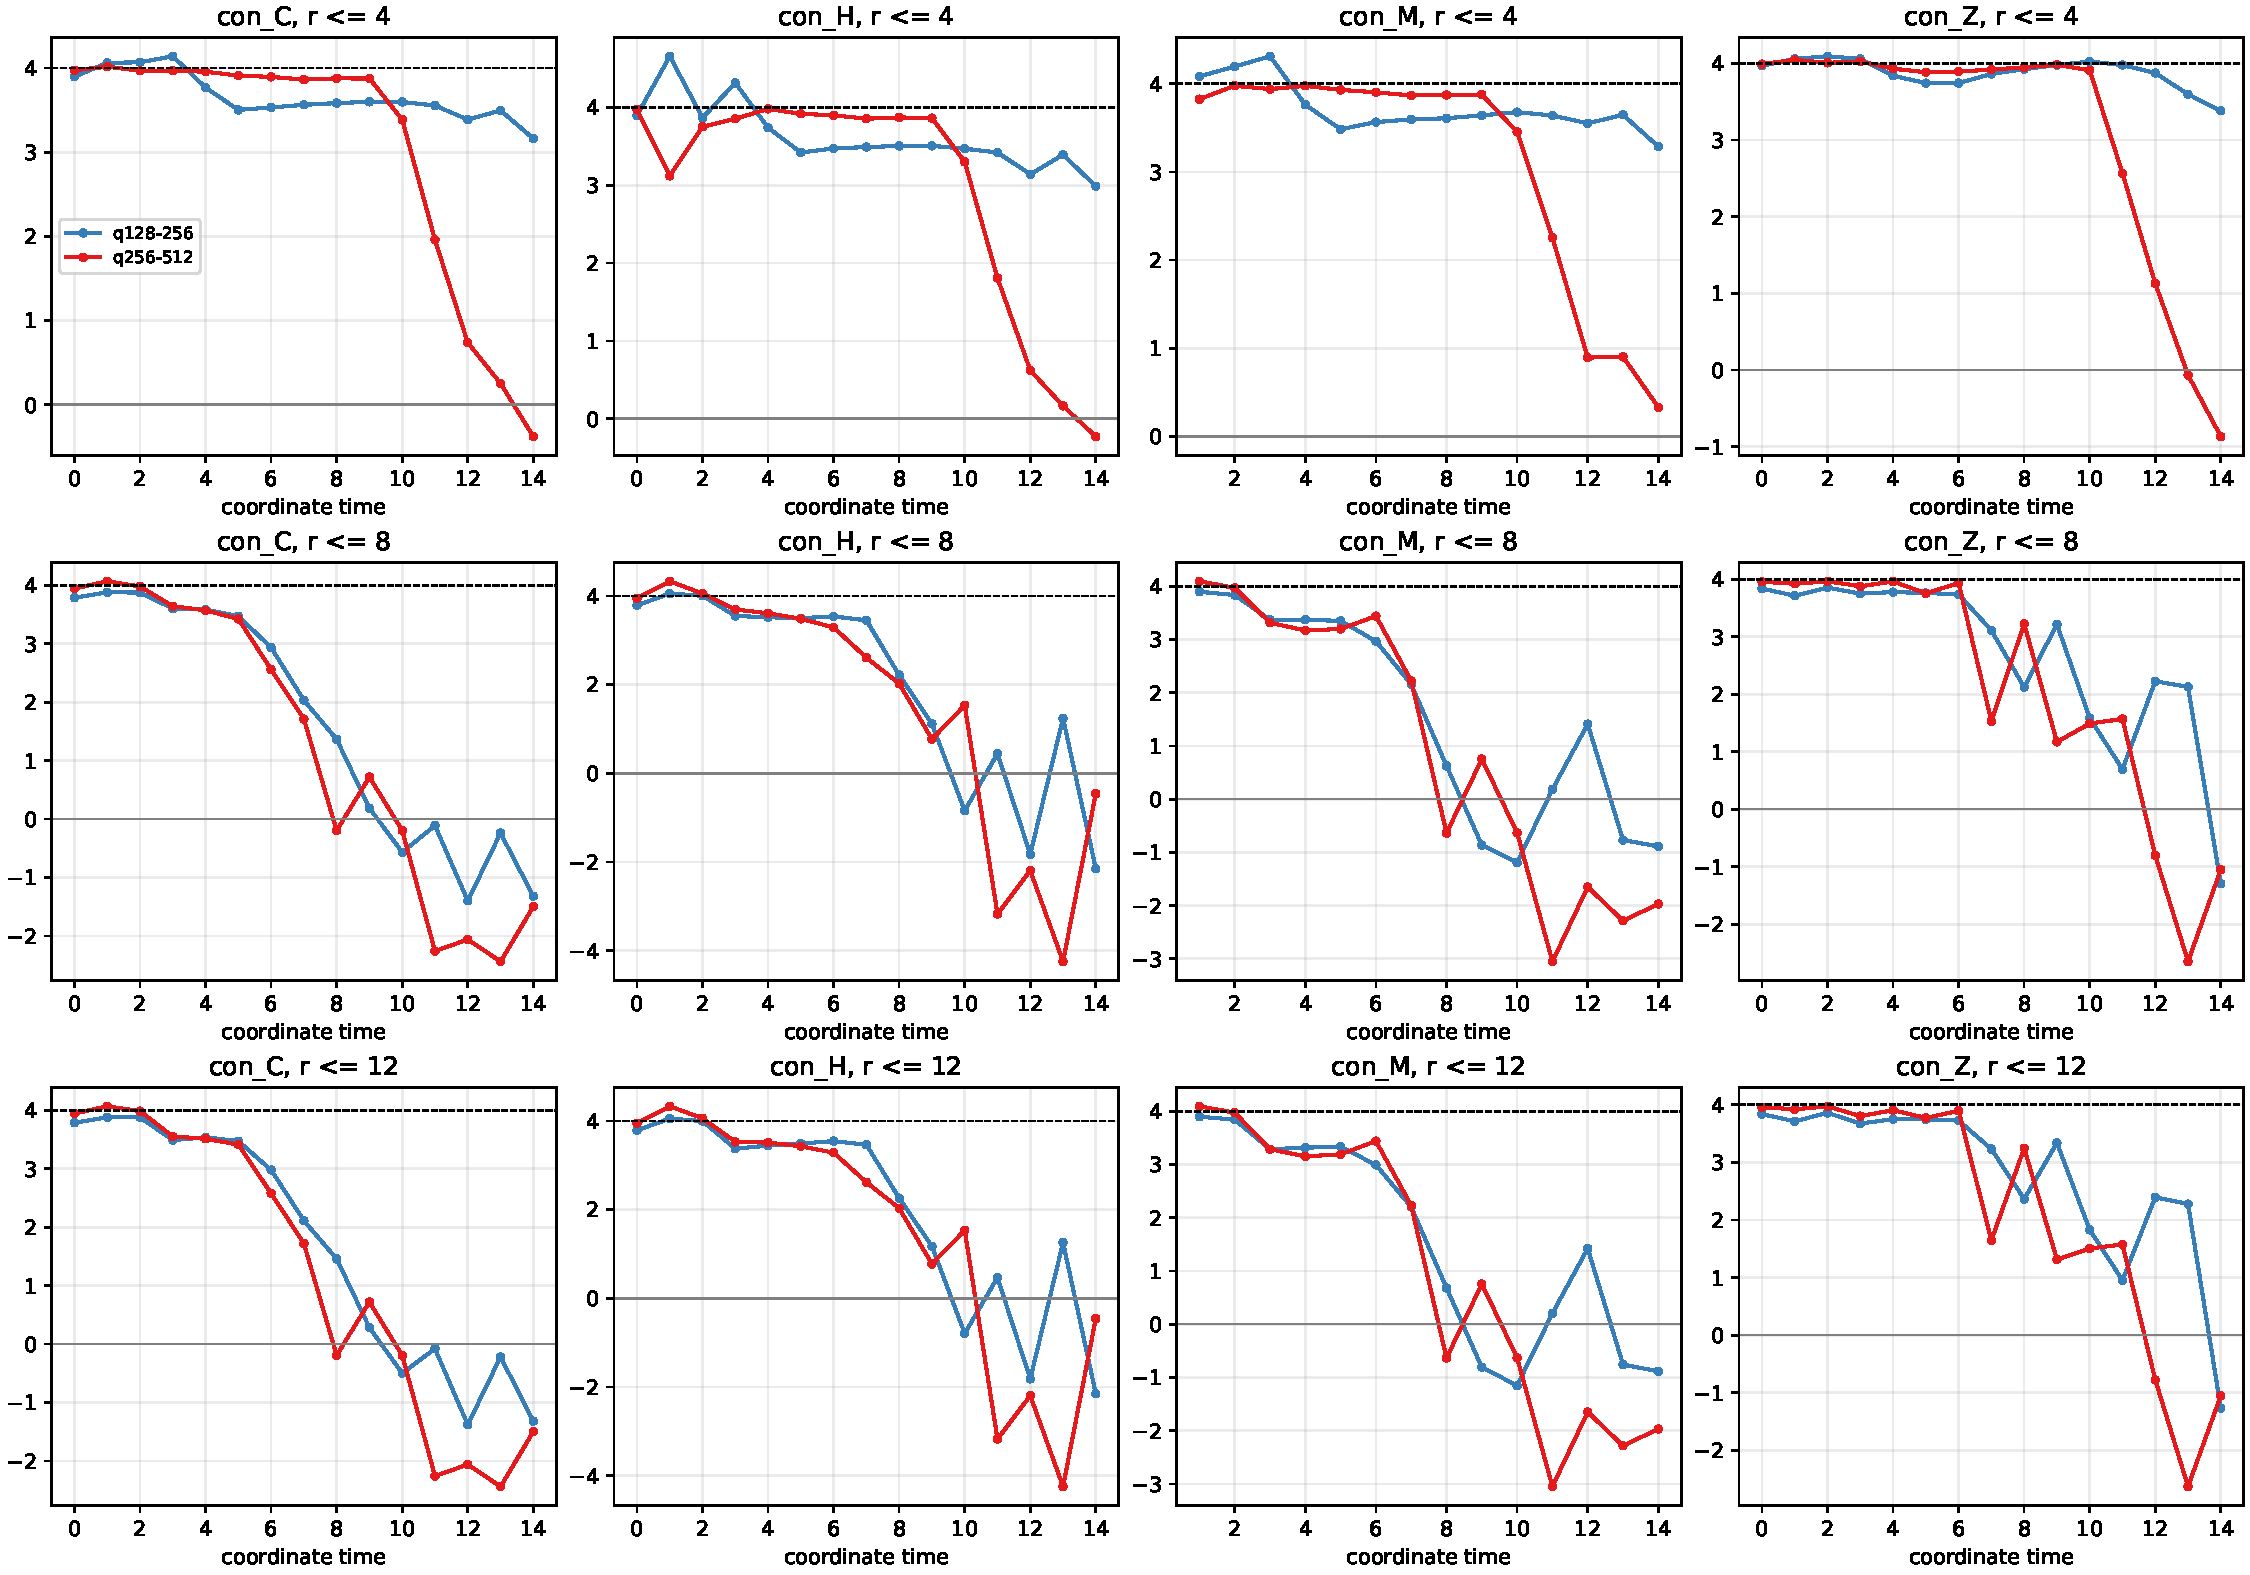
\includegraphics[width=.82\linewidth]{analysis/regional_constraints/figures/regional_constraint_orders.pdf}
\caption{Pairwise amplitude orders on the matched common lattice. The diagnostic
filters scales below $h=0.25$ and is not the native leaf quadrature.}
\end{figure}

\clearpage
\section*{Experimental Bjorhus compatibility boundary}
A concrete frame-construction bug was found and repaired: raised normal
components consumed not-yet-initialized covariant components for non-diagonal
metrics. Commit \texttt{d39822c6522688749fe5ead8025907bc055f02f8}
separates initialization and index raising and adds a regression test. The
strict residual gate was not weakened, and final CUDA tests pass.

The planned A/B/C/D discriminator is incomplete. A (Rout16 original) and C
(Rout128 original) reached $t=6.5M$. B (Rout16 CPBC) developed a corner-local
runaway and failed at $t=3.244461M$. D was intentionally cancelled at
$t=1.508791M$ and is excluded. The current CPBC is not production-stable, and
no claim of boundary-error reduction is supported.

\begin{figure}[ht]
\centering
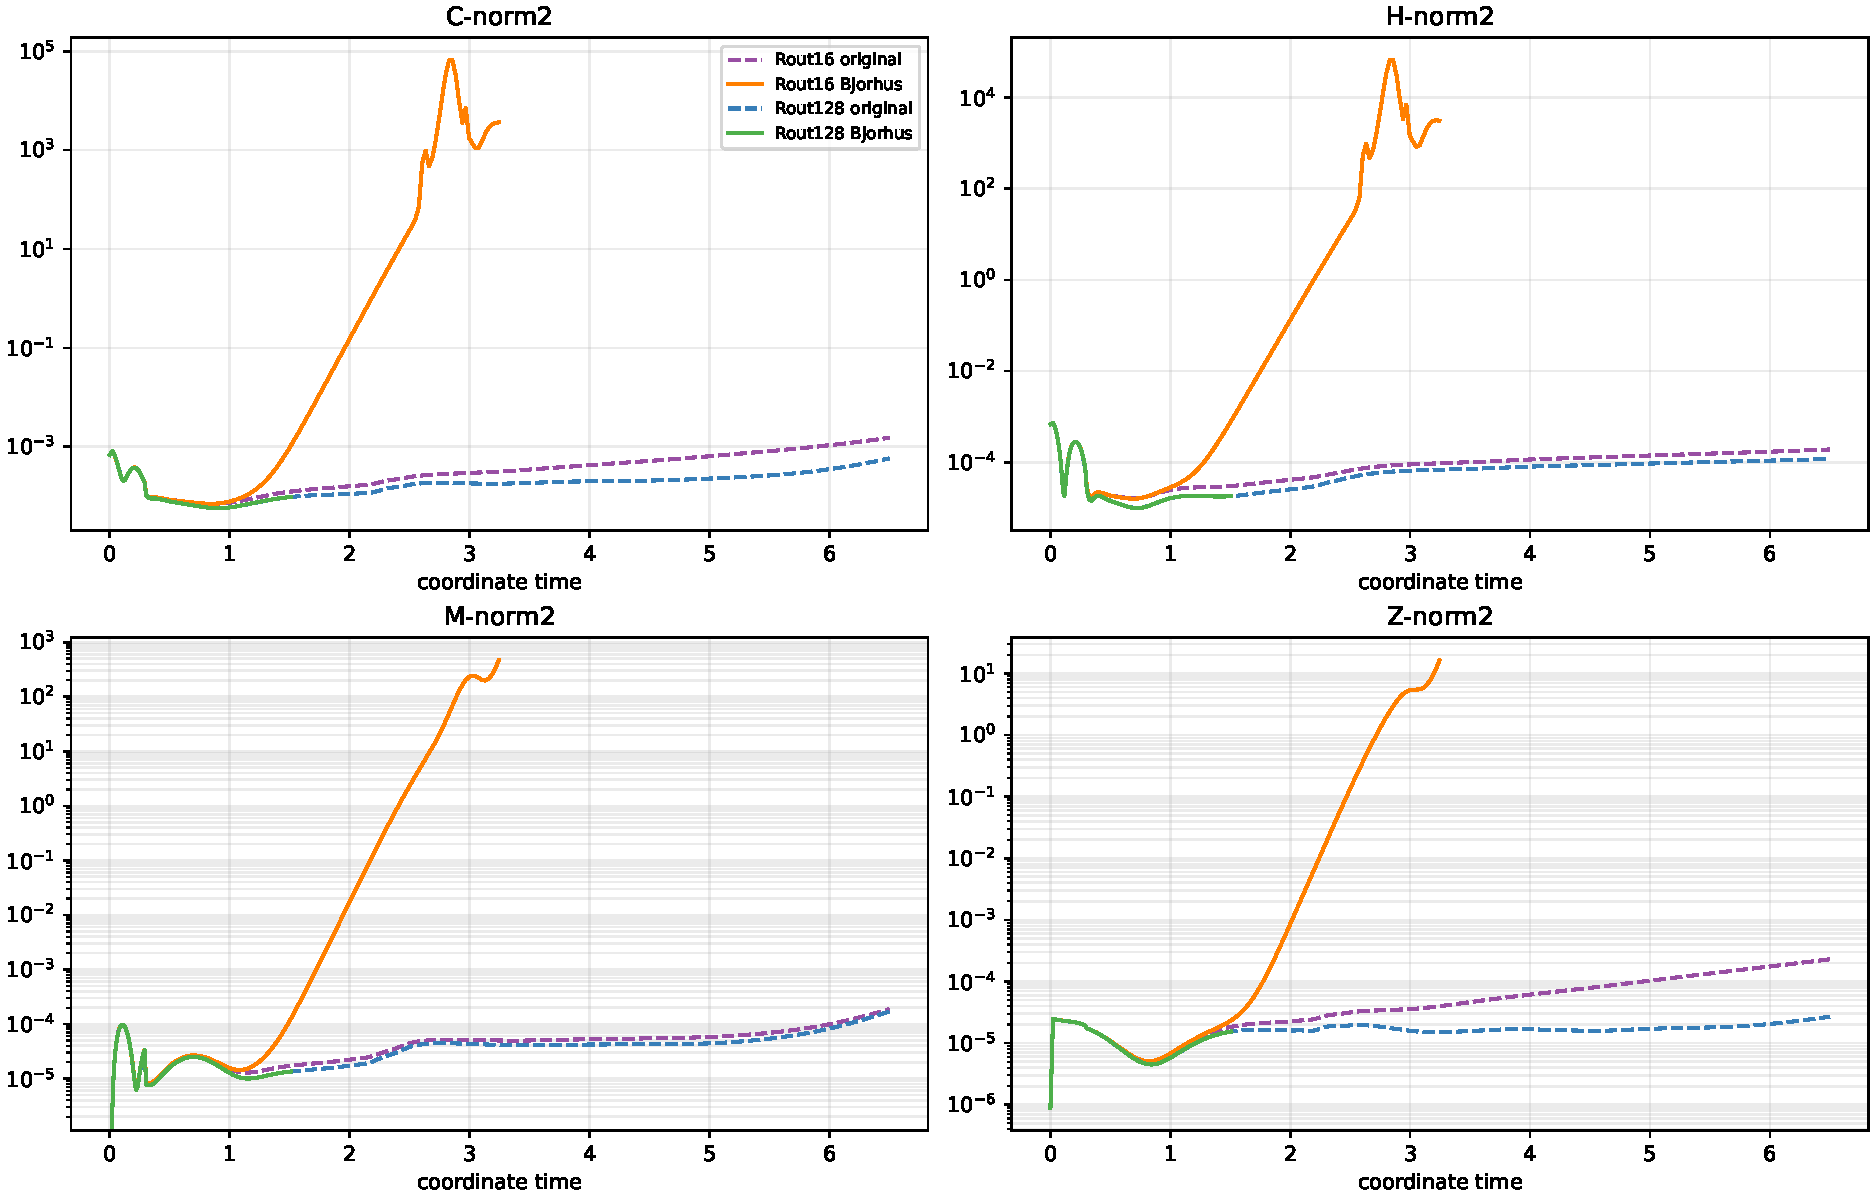
\includegraphics[width=.82\linewidth]{analysis/cpbc/figures/cpbc_constraint_histories.pdf}
\caption{Retained boundary discriminator histories. D is partial and excluded;
the four-way comparison is not qualified.}
\end{figure}

\section*{Claim boundary and next step}
Current evidence strongly deprioritizes the physical outer boundary and Cartoon
axis relative to a bulk/AMR high-frequency or interface mechanism near
$\rho\simeq5M$, but does not mathematically exclude boundary effects or isolate
a unique source bug. No t=30 stability, Figure-3 reproduction, convergence,
horizon, or critical-phenomena claim is made. The smallest next action should
be a bounded stage-resolved diagnostic around the first loss of regional
convergence, not a long evolution or broad parameter sweep.

Full paths, hashes, limitations, and compact CSV evidence are recorded in
\texttt{EVIDENCE\_MANIFEST.json} and the accompanying Markdown reports.
\end{document}
